%% Slides for ".NET Programming" by Chunyu Wang <chunyu@hit.edu.cn>

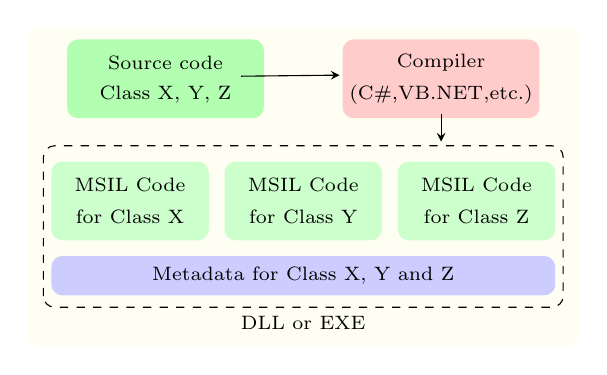
\begin{tikzpicture}[font=\scriptsize, rounded corners, >=stealth]
\path[fill=yellow!10,fill opacity=.5] (1.5,.85) rectangle (8.5,4.9);
\path[fill=green!30] (2,3.75) rectangle +(2.5,1) 
+(1.25,.3) node (a) {Class X, Y, Z} +(1.25,.7) node {Source code};
\path[fill=red!20] (5.5,3.75) rectangle +(2.5,1) 
+(1.25,.3) node (b) {(C\#,VB.NET,etc.)} +(1.25,.7) node {Compiler};
\draw[->] (a.north east) -- (b.north west);
\draw[->] (b.south) -- +(down:.35cm);
\draw[dashed,fill=yellow!5] (1.7,1.35) rectangle (8.3,3.4) (5,1.15) node {DLL or EXE};
\foreach \x/\y in {-2.2cm/X,0cm/Y,2.2cm/Z} 
\path[fill=green!20,xshift=\x] (4,2.2) rectangle +(2,1) +(1,.7) node {MSIL Code} +(1,.3) node {for Class \y} ;
\path[fill=blue!20] (1.8,1.5) rectangle +(6.4,.5) +(3.2,.25) node {Metadata for Class X, Y and Z};
\end{tikzpicture}
